% Author : Alexandre Quenon
% Last update : July 5, 2014

% % % % % % %
%  Packages %
% % % % % % %

%---Base packages
\documentclass[t]{beamer}			% document type
	% options are:
		% c or t to place the text at the vertical center or top of the slides
	% some packages are automatically loaded: 
		% amsmath, amsthm, amssymb; color, xcolor; hyperref
\usepackage[utf8]{inputenc}			% encoding
\usepackage[T1]{fontenc}			% accent
\usepackage{lmodern}				% latin font

%---Language(s)
\usepackage[english,frenchb]{babel}	% last language = typography by default
\addto\captionsfrench{				% to change the french names of...
	\renewcommand{\tablename}{\textsc{Tableau}}	% (default \textsc{Table})
}

%---Slide layout
%------> Browsing bar
	\setbeamertemplate{navigation symbols}{}	% to remove the browsing bar
%------> UMONS template
	\usetheme[navigation,no-subsection,no-totalframenumber]{UMONS}
	\title{Big Data I - présentation de projet}
	\subtitle{Construction d'un modèle de prédiction}
	\author[shortname]{Rémy \textsc{Decocq} \and Sam \textsc{Boosko} \and Dimitri \textsc{Waelkens}}
	\date{20 mai 2019}
	\institute[| shortFac]{%
	  Faculté des Sciences\\
	  Université de Mons
	  \\[4ex]
	  
\includegraphics[height=6ex]{umonsLogos/UMONS-Logo}\hspace{2em}%
	  \raisebox{-1ex}{
\includegraphics[height=8ex]{umonsLogos/FS-Logo}}
	}

%---Floating objects (images, tables,...)
\usepackage{float}					% better management of floating objects
\usepackage{array}					% better management of tables
\usepackage{graphicx}				% to include external images
\graphicspath{{Images/}}			% to put images in an 'Images' folder 
%\usepackage{caption}				% /!\ has priority on "memoir" class
%\usepackage{subcaption}			% subfigure and subtable environments
%\usepackage{subfig}				% \subfloat command
%\usepackage{wrapfig}				% wrapfigure environment
%\usepackage[update]{epstopdf}		% to use '.eps' files with PDFLaTeX

%---Code including
%\usepackage{listings}				% general package (can be tuned)
%\usepackage[framed]{mcode}			% to include Matlab code
									% /!\ you need the "mcode.sty" file

%---Units from International System
\usepackage{siunitx}				% \SI{}{} command (units with good typography)
\DeclareSIUnit\baud{baud}			% definition of the "baud" unit
\DeclareSIUnit\bit{bit}				% definition of the "bit" unit

%---Drawing
%\usepackage{tikz}					% useful package for drawing
%\usepackage[european]{circuitikz} 	% to draw electrical circuits

%---Amsthm
%\theoremstyle{plain}% default
%\newtheorem{thm}{Theorem}
%\newtheorem{lem}[thm]{Lemma}
%\newtheorem{prop}[thm]{Proposition}
%\newtheorem*{cor}{Corollary}
%
%\theoremstyle{definition}
%\newtheorem{defn}{Definition}[section]
%\newtheorem{conj}{Conjecture}[section]
%\newtheorem{exmp}{Example}[section]
%
%\theoremstyle{remark}
%\newtheorem*{rem}{Remark}
%\newtheorem*{note}{Note}
%\newtheorem{case}{Case}

% % % % % % %
% Document	%
% % % % % % %

\begin{document}
% Title page & Outline
% --------------------
	\frame[plain]{\titlepage}
	
	\frame{
		\tableofcontents
	}
					% to insert the toc at each new section
% Presentation
% ------------
	\section{Introduction}
	\subsection{Ensemble de données}
	\frame{
		\frametitle{Introduction}	% Sommaire
		\framesubtitle{Ensemble de données}
		\begin{itemize}
		\item{Les données se présentent sous la forme d'un tableau contenant des informations relatives à un individu. \\
		
		\begin{figure}[h!]
			\begin{tabular}{|c|c|c|c|c|c|}
			\hline
			& \textbf{Age} & \textbf{job} & \textbf{marital} & \textbf{...} & \textbf{y}\\
			\hline
			1		& 56  & housemaid 	& married 	& ... & 0\\
			2		& 57  & services 	& married 	& ... & 0\\
			3		& 37  & services 	& married 	& ... & 0\\
			... 	& ... & ... 		& ... 		& ... & ...\\
			30436 	& 61  & retired 	& married  	& ... & 0\\
			\hline
			\end{tabular}
			\caption{Dataset Dtrain.csv}
		\end{figure}}
		\item{Où la variable y vaut $\begin{cases} 1 \text{ si cet individu a ouvert un compte en banque} \\0 \text{ sinon}\end{cases}$}
		\end{itemize}
	}
	\subsection{Sélection du type de modèle}
	\frame{
		\frametitle{Introduction}
		\framesubtitle{Sélection du type de modèle}
		\begin{itemize}
		\item{Au vu des données et de la prédiction recherchée, nous pouvons en déduire qu'il s'agit d'un problème de \textbf{classification}.}
		\item{2 méthodes de classifications vue au cours testées:
			\begin{enumerate}
			\item{\textbf{Logistic Regression}}
			\item{Linear Discriminant Analysis (LDA)}	
			\end{enumerate}}
		\item{\textbf{LDA} est plus \textbf{stable} quand les prédicteurs suivent une \textbf{distribution gaussienne}. Or, les données n'ont pas cette distribution.}
		\item{Donnant de \textbf{meilleurs résultats}, la \textbf{régression logistique} a été retenue.}
		\end{itemize}			
	}	
	\section{Analyse et preprocessing du dataset}
	\subsection{Analyse du dataset}
	\frame{
	    \frametitle{Analyse et preprocessing du dataset}
		\framesubtitle{Analyse du dataset}
		\begin{itemize}
		\item{L'analyse des données montre:
			\begin{enumerate}
				 \item{seulement \textbf{3} observations de \textbf{default} valent \textit{yes} sur \textbf{30436}.}
				 \item{le nombre de \textbf{1} n'est pas proportionnel au nombre de \textbf{0}}
				 \item{il y a \textbf{1316} observations où
				 	\[
				 		pdays = 999 \land previous \geq 1
				 	\]
				 	dont \textbf{108} se rapportent à \textbf{y = 1}}
			\end{enumerate}}
		\end{itemize}
		
		\begin{figure}[h!]
			\begin{minipage}[c]{.46\linewidth}
				\begin{figure}[h!]\begin{tabular}{|c|c|c|}
				\hline
				\textbf{yes} & \textbf{no} & \textbf{unknown}\\
				\hline
				3 & 7532 & 22901\\
				\hline
				\end{tabular}
				\caption{table of people\$default}
				\end{figure}
			\end{minipage} \hfill
			\begin{minipage}[c]{.46\linewidth}
				\begin{figure}[h!]\begin{tabular}{|c|c|c|}
				\hline
				\textbf{1} & \textbf{0} & \textbf{total}\\
				\hline
				2342 & 28094 & 30436\\
				\hline
				\end{tabular}
				\caption{table of people\$y}
				\end{figure}
			\end{minipage}
		\end{figure}
	}
	\subsection{Preprocessing du dataset}
	\frame{
	    \frametitle{Analyse et preprocessing du dataset}
		\framesubtitle{Sélection des observations pour le training et la validation}
	    \begin{figure}[h!]
  		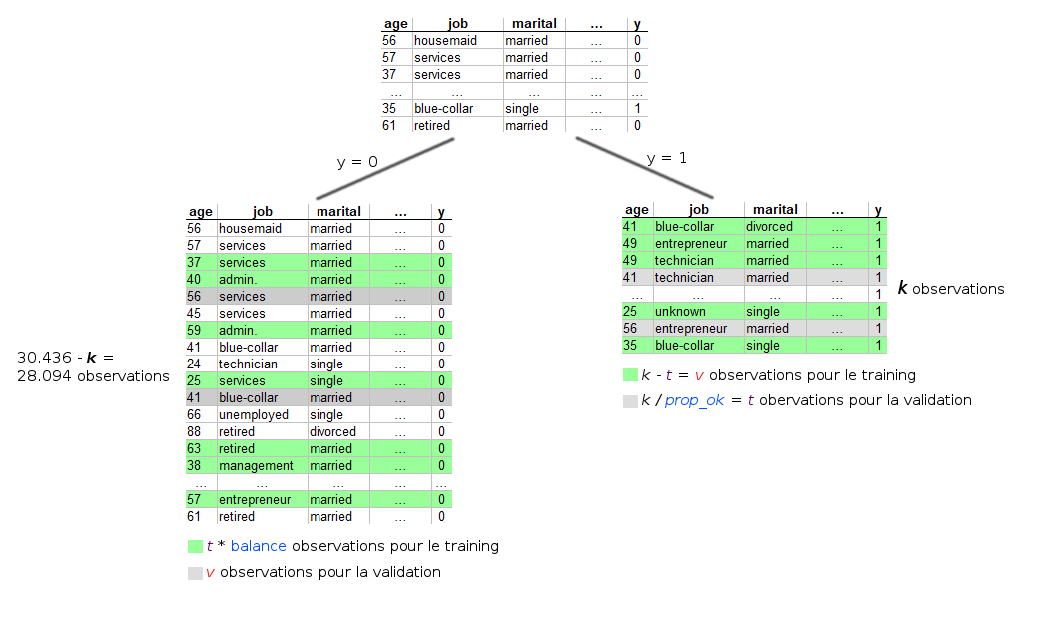
\includegraphics[scale=0.43]{img/a/pastedf.PNG}
		\end{figure}
	}	
	
	\frame{
		\frametitle{Analyse et preprocessing du dataset}
		\framesubtitle{Preprocessing du dataset}
		\begin{itemize}
		\item{Catégorisation des valeurs des variables \textbf{job} et \textbf{pdays}.
			\begin{itemize}
			\item{\textbf{jobs}:
			 $poor = \begin{cases}blue-collar \\ housemaid \\ services \\ technician \\ unknown\end{cases}$,
			 $middle = \begin{cases}admin. \\ entrepreneur \\ management \\ self-employed \\ unemployed\end{cases}$,
			 $good = \begin{cases}retired \\ student\end{cases}$\\
			 }
			\item{\textbf{pdays}: 999 = never, > 5 = late, $\leq$ 5 = recent}
			\end{itemize}}
		\end{itemize}
	}	
	\subsection{Sélection des prédicteurs}
	\frame{
		\frametitle{Analyse et preprocessing du dataset}
	    \framesubtitle{Sélection des prédicteurs}
	    \begin{itemize}
	    \item{Analyse de la signification des variables avec \textbf{stepwise selection}.
	    	\begin{figure}[h!]
  			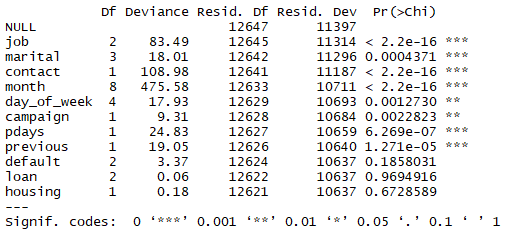
\includegraphics[scale=0.7]{img/anal1.PNG}
			\end{figure}}
		\item{3 \textbf{variables} ne sont pas \textbf{significatives}:
		\begin{enumerate}
		\item default
		\item loan
		\item housing
		\end{enumerate}}
		\end{itemize}
	}
	
	\section{Résultats du modèle}
	\frame{
		\frametitle{Résultats du modèle}
		\begin{itemize}
		\item{Les résultats ont été obtenus sur des ensembles donnés par \textbf{SepDataSet} avec les paramètres:
			\begin{itemize}
			\item{$prop\_ok = 10$}
			\item{$balance = 5$}
			\end{itemize}}
		\end{itemize}
		\begin{figure}
		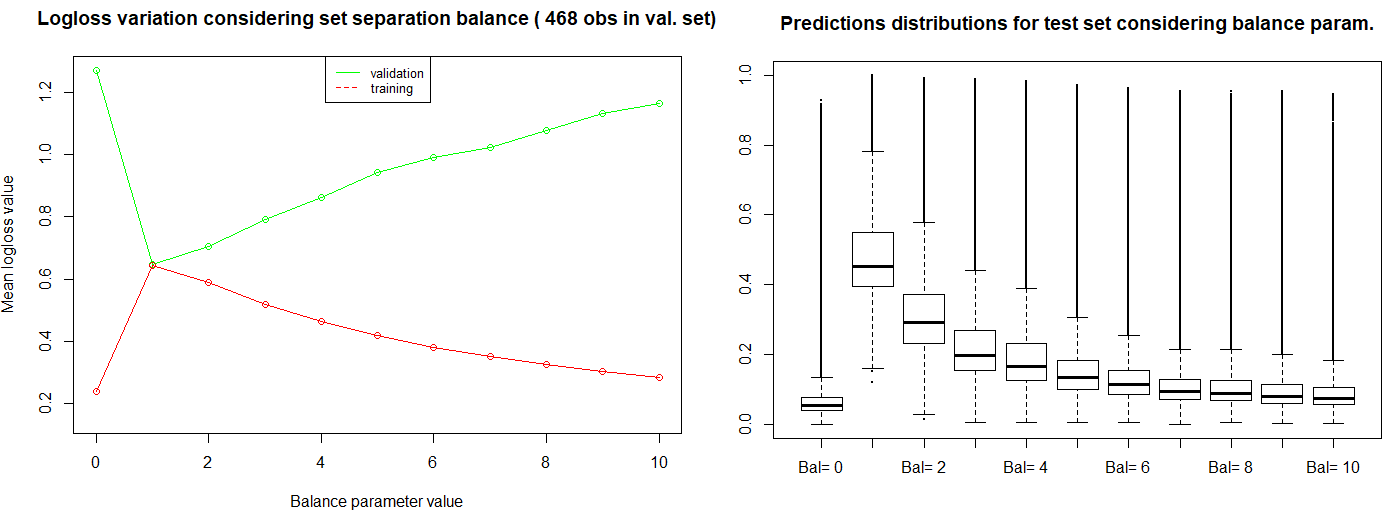
\includegraphics[scale=0.24]{img/balance_both.PNG}
		\end{figure}
	}	
	
	\frame{
	    \frametitle{Résultats du modèle}
	    \begin{itemize}
	    \item{Ce modèle fait l'\textbf{hypothèse} que la \textbf{relation} avec la \textbf{variable} expliquée est \textbf{linéaire}.}
	    \item{Calcul des prédictions sur:
			\begin{enumerate}
			\item{les données du \textbf{training set} où de l'\textbf{overfitting} est observable.
			\begin{figure}[h!]
  			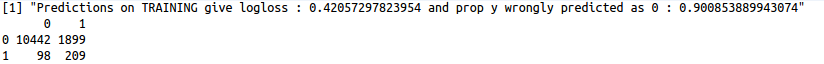
\includegraphics[scale=0.45]{img/predtr.PNG}
  			\caption{Training Set Confusion Matrix}
			\end{figure}}
			\item{les données du validation set.
			\begin{figure}[h!]
  			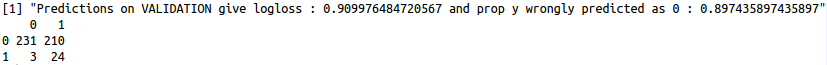
\includegraphics[scale=0.45]{img/predva.PNG}
  			\caption{Validation Set Confusion Matrix}
			\end{figure}}
			\end{enumerate}}
	    \item{Cette \textbf{classification} a été effectuée considérant un \textbf{seuil} de \textbf{0.5} .}
	    \end{itemize}
	}
	
	\frame{
		\frametitle{Résultats du modèle}
		\begin{figure}
		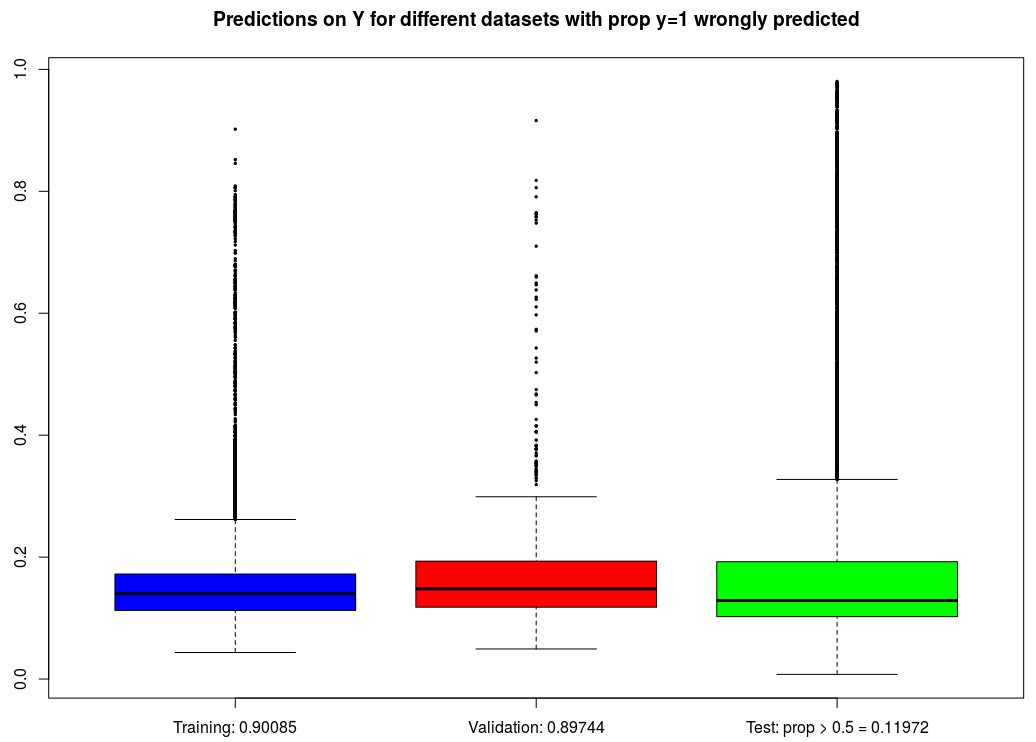
\includegraphics[scale=0.28]{img/pred_distrib.PNG}
		\end{figure}			
	}		
	
	\section{Cross-Validation de la procédure}
	\frame{
	    \frametitle{Cross-Validation de la procédure}
	    \begin{itemize}
	    \item{La procédure de cross-validation va permettre:
			\begin{enumerate}
			\item{d'estimer l'erreur de test.}
			\item{de mettre en évidence la stabilité du modèle.}			
			\end{enumerate}}
	    \end{itemize}
	    \begin{figure}[h!]
  			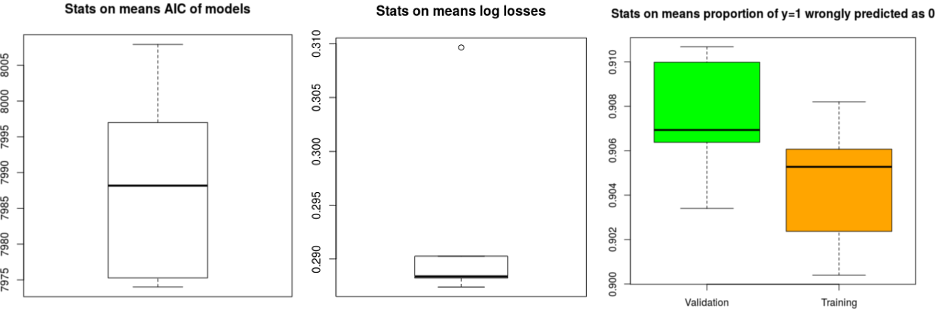
\includegraphics[scale=0.35]{img/cv.PNG}
		\end{figure}
	}
	
	\section{Conclusion}
	\frame{
	    \frametitle{Conclusion}
	    \begin{itemize}
	    \item{Un modèle de \textbf{classification} a été sélectionné, la \textbf{régression logistique}.}
	    \item{Une procédure, \textbf{paramétrée} avec $prop\_ok = 10$ et $balance = 5$, de \textbf{sélection des observations} a été effectuée afin d'avoir une \textbf{meilleure proportion d'observations} où y = 0 par rapport au nombre d'observations où y = 1. }
	    \item{Sélection des variables significatives par la méthode \textbf{stepwise selection}}
	    \item{\textbf{Logloss} de \textbf{0.55 à 0.52} sur le dataset en ligne sur \textbf{kaggle.com} .}
	    \end{itemize}
	}

\end{document}
